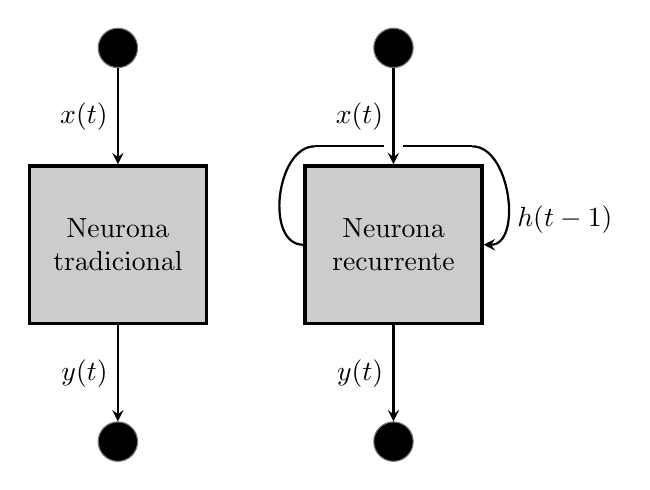
\begin{tikzpicture}
	\tikzstyle{box} = [draw,inner sep=7,minimum size=57,line 
			width=1, very thick, draw=black, fill=black!20, text width=50pt, text centered]
	\tikzstyle{stealth} = [-stealth, thick]
	\tikzstyle{invisible} = [outer sep=0,inner sep=0,minimum size=0]
	\tikzstyle{circle} = [shape=circle, minimum size=0.5cm, draw=black!55]
	\tikzstyle{line} = [draw, very thick, red]

	\begin{scope}
	\node [box] (v2) at (0,0) {Neurona tradicional};
	\node [circle, fill] (v1) at (0,2.5) {};
	\node [circle, fill] (v3) at (0,-2.5) {};
	\draw [stealth] (v1) edge node[anchor=east] {$x(t)$} (v2);
	\draw [stealth] (v2) edge node[anchor=east] {$y(t)$} (v3);
	\end{scope}
	\begin{scope}[shift={(3.5,0)}]
	\node [box] (v2_1) at (0,0) {Neurona recurrente};
	\node [circle, fill] (v1_1) at (0,2.5) {};
	\node [circle, fill] (v3_1) at (0,-2.5) {};
	\draw [stealth] (v1_1) edge node [anchor=east] {$x(t)$} (v2_1);
	\draw [stealth] (v2_1) edge node [anchor=east] {$y(t)$} (v3_1);
	\end{scope}

\node [invisible, anchor=east] (v5) at (4.5,1.25) {};
\draw [stealth, in =0, out=0] (v5) edge node[anchor=north west] {$h(t-1)$} (v2_1);
\node [invisible] (v4) at (2.5,1.25) {};
\node [] (v6) at (3.5,1.25) {};
\draw [thick, in =180, out=180] (v2_1) edge (v4);
\draw [thick] (v4) edge (v6);
\draw [thick] (v6) edge (v5);
\end{tikzpicture}